% coding:utf-8

%----------------------------------------
%FOSAMATH, a LaTeX-Code for a mathematical summary for basic analysis
%Copyright (C) 2013, Daniel Winz, Ervin Mazlagic, Adrian Imboden, Philipp Langer

%This program is free software; you can redistribute it and/or
%modify it under the terms of the GNU General Public License
%as published by the Free Software Foundation; either version 2
%of the License, or (at your option) any later version.

%This program is distributed in the hope that it will be useful,
%but WITHOUT ANY WARRANTY; without even the implied warranty of
%MERCHANTABILITY or FITNESS FOR A PARTICULAR PURPOSE.  See the
%GNU General Public License for more details.
%----------------------------------------

% coding:utf-8
\section{Aufgabe mit Fourierreihen}
Gegeben ist die Funktion: 
\[ f(x) = \left\{\begin{array}{ll}
0     &\text{für } x=0\\
1 - x &\text{für } 0 < x \leq 1\\
0     &\text{für } 1 < x \leq 2
\end{array}\right. \]
auf dem Intervall $[0,2]$\\\\
a)\\
Skizzieren Sie den Graph der Funktion $f$. 
\begin{figure}[h!]
\centering
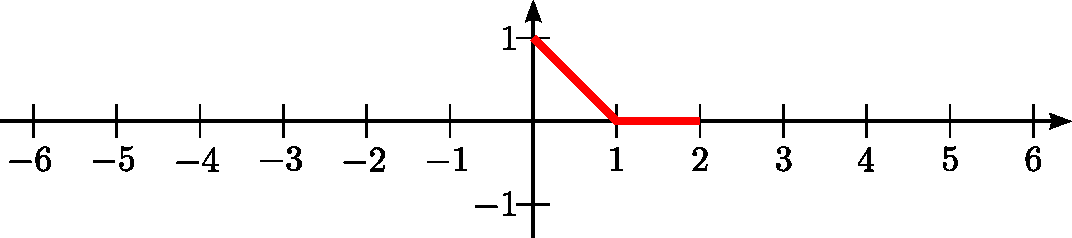
\includegraphics[width=1\textwidth]{fourier0.pdf}
\end{figure}

b)\\
Die Funktion soll zu einer ungeraden Funktion mit Periodenlänge 4 fortgesetzt werden. Machen Sie davon eine Skizze im Bereich $-6 \leq x \leq 6$.\\\\
\begin{figure}[h!]
\centering
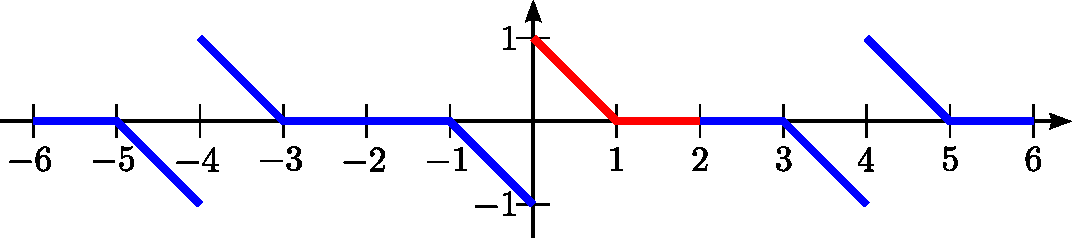
\includegraphics[width=1\textwidth]{fourier1.pdf}
\end{figure}

c)\\
Berechnen Sie die Koeffzienten $a_n$ und $b_n$ der Fourier Reihe dieser periodischen Funktion in allgemeiner Form.\\\\
\[ \left. \begin{matrix}
a_0 = 0\\
a_k = 0
\end{matrix} \right\} \text{weil $f(x)$ ungerade} \]
\[ b_k = \frac{2}{T} \int_{T}^{} f(x) \sin\left(\frac{2 \pi}{T} K x\right) dx \]
\[ b_k = \frac{2}{4} \int_{-2}^{2} f(x) \sin\left(\frac{2 \pi}{4} K x\right) dx \]
\[ b_k = \int_{0}^{1} f(x) \sin\left(\frac{\pi}{2} K x\right) dx \]
\[ b_k = \int_{0}^{1} (1 - x) \sin\left(\frac{\pi}{2} K x\right) dx \]
\[ b_k = \int_{0}^{1} \underbrace{\sin\left(\frac{\pi}{2} K x\right) dx}_{\left.-\cos\left(\frac{\pi}{2}K x\right) \cdot \frac{2}{\pi K}\right|_0^1} - \underbrace{\int_{0}^{1} x \sin\left(\frac{\pi}{2} K x\right) dx}_{\text{partiell integrieren}} \]
Partielle Integration von $\int_{0}^{1} x \sin\left(\frac{\pi}{2} K x\right) dx$: 
\[ \int_{0}^{1} x \sin\left(\frac{\pi}{2} K x\right) dx = \left.-\cos\left(\frac{\pi}{2}Kx\right) \cdot \frac{2}{\pi K} \cdot x\right|_0^1 - \int_{0}^{1} -\cos\left(\frac{\pi}{2}Kx\right) \cdot \frac{2}{\pi K} dx \]
\[ = \left.-\cos\left(\frac{\pi}{2}Kx\right) \cdot \frac{2}{\pi K} \cdot x\right|_0^1 - \frac{2}{\pi K} \cdot \int_{0}^{1} -\cos\left(\frac{\pi}{2}Kx\right)  dx \]
\[ = \left.-\cos\left(\frac{\pi}{2}Kx\right) \cdot \frac{2}{\pi K} \cdot x\right|_0^1 - \left.\frac{2}{\pi K} \cdot \left(-\sin\left(\frac{\pi}{2}Kx\right)\frac{2}{\pi K}\right)\right|_0^1 \]
\[ = \left.-\cos\left(\frac{\pi}{2}Kx\right) \cdot \frac{2}{\pi K} \cdot x\right|_0^1 + \left.\frac{4}{\pi^2 K^2} \cdot \left(\sin\left(\frac{\pi}{2}Kx\right)\right)\right|_0^1 \]
\[ = -\left(\cos\left(\frac{\pi}{2}K \cdot 1\right) \cdot \frac{2}{\pi K} \cdot 1 - \underbrace{\cos\left(\frac{\pi}{2}K \cdot 0\right) \cdot \frac{2}{\pi K} \cdot 0}_0\right) + 
\left.\frac{4}{\pi^2 K^2} \cdot \left(\sin\left(\frac{\pi}{2}Kx\right)\right)\right|_0^1 \]
\[ = -\left(\cos\left(\frac{\pi}{2}K\right) \cdot \frac{2}{\pi K} \cdot 1 - 0\right) + 
\left.\frac{4}{\pi^2 K^2} \cdot \left(\sin\left(\frac{\pi}{2}Kx\right)\right)\right|_0^1 \]
\[ = -\left(\cos\left(\frac{\pi}{2}K\right) \cdot \frac{2}{\pi K} \cdot 1\right) + 
\left(\frac{4}{\pi^2 K^2} \cdot \left(\sin\left(\frac{\pi}{2}K \cdot 1\right)\right) - \underbrace{\frac{4}{\pi^2 K^2} \cdot \left(\sin\left(\frac{\pi}{2}K \cdot 0\right)\right)}_0\right) \]
\[ = -\left(\cos\left(\frac{\pi}{2}K\right) \cdot \frac{2}{\pi K} \cdot 1\right) + 
\left(\frac{4}{\pi^2 K^2} \cdot \left(\sin\left(\frac{\pi}{2}K \cdot 1\right)\right) - 0\right) \]
\[ = -\left(\cos\left(\frac{\pi}{2}K\right) \cdot \frac{2}{\pi K}\right) + 
\left(\frac{4}{\pi^2 K^2} \cdot \left(\sin\left(\frac{\pi}{2}K\right)\right)\right) \]
Ergebniss aus der partiellen Integration wieder einsetzen: 
\[ b_k = \left(\left.-\cos\left(\frac{\pi}{2}K x\right) \cdot \frac{2}{\pi K}\right|_0^1 \right) - \left(-\left(\cos\left(\frac{\pi}{2}K\right) \cdot \frac{2}{\pi K}\right) + \left(\frac{4}{\pi^2 K^2} \cdot \left(\sin\left(\frac{\pi}{2}K\right)\right)\right)\right) \]
\[ b_k = \left(\left(-\cos\left(\frac{\pi}{2}K \cdot 1\right) \cdot \frac{2}{\pi K} - \underbrace{-\cos\left(\frac{\pi}{2}K \cdot 1\right) \cdot \frac{2}{\pi K}}_{-\frac{2}{\pi K}}\right) \right)- \left(-\left(\cos\left(\frac{\pi}{2}K\right) \cdot \frac{2}{\pi K}\right) + \left(\frac{4}{\pi^2 K^2} \cdot \left(\sin\left(\frac{\pi}{2}K\right)\right)\right)\right) \]
\[ b_k = \left(-\cos\left(\frac{\pi}{2}K \cdot 1\right) \cdot \frac{2}{\pi K} + \frac{2}{\pi K}\right) + \left(\cos\left(\frac{\pi}{2}K\right) \cdot \frac{2}{\pi K}\right) - \left(\frac{4}{\pi^2 K^2} \cdot \left(\sin\left(\frac{\pi}{2}K\right)\right)\right) \]
\[ b_k = -\cos\left(\frac{\pi}{2}K \cdot 1\right) \cdot \frac{2}{\pi K} + \frac{2}{\pi K} + \cos\left(\frac{\pi}{2}K\right) \cdot \frac{2}{\pi K} - \left(\frac{4}{\pi^2 K^2} \cdot \left(\sin\left(\frac{\pi}{2}K\right)\right)\right) \]
\[ \underline{b_k = \frac{2}{\pi K} - \frac{4}{\pi^2 K^2} \cdot \sin\left(\frac{\pi}{2}K\right)} \]
Fourierreihe hinschreiben
\[ f_n(x) = \frac{a_0}{2} + \sum_{K=1}^{n}\left(a_k \cdot \cos \left(\frac{2 \pi}{T}Kx\right) + b_k \cdot \sin\left(\frac{2 \pi}{T}Kx\right)\right) \]
\[ f_n(x) = \frac{0}{2} + \sum_{K=1}^{n}\left(0 \cdot \cos \left(\frac{2 \pi}{T}Kx\right) + b_k \cdot \sin\left(\frac{2 \pi}{T}Kx\right)\right) \]
\[ f_n(x) = \sum_{K=1}^{n}\left(b_k \cdot \sin\left(\frac{2 \pi}{T}Kx\right)\right) \]
\[ f_n(x) = \sum_{K=1}^{n}\left(\left(\frac{2}{\pi K} - \frac{4}{\pi^2 K^2} \cdot \sin\left(\frac{\pi}{2}K\right)\right) \cdot \sin\left(\frac{2 \pi}{T}Kx\right)\right) \]
% \[  \]
% \[  \]
% \[  \]
% \[  \]
% \[  \]
% \[  \]

% d)\\
% Berechnen Sie die Fourierkoeffzienten in numerischer Form (2. St. n. d.
% Komma) und schreiben Sie die Fourier Reihe bis und mit der 4. Oberschwingung (Kreisfrequenz $4\omega$) auf.